\documentclass[tikz,border=3pt]{standalone}
\usepackage[utf8]{inputenc}
\usepackage[T1]{fontenc}
\usepackage{lmodern}
\renewcommand{\familydefault}{\sfdefault}
\usepackage{sansmath}\sansmath
\usepackage{chemfig}
\usepackage{pgfplots}\pgfplotsset{compat=1.18,/pgf/number format/use comma,/pgf/number format/1000 sep={.}}
\usetikzlibrary{arrows.meta,calc,positioning,decorations.pathmorphing,patterns}
% paleta del sitio
\definecolor{nar}{HTML}{E8680C}\definecolor{narc}{HTML}{FFB35C}\definecolor{hielo}{HTML}{FFF3E8}
\definecolor{tinta}{HTML}{1D1D1F}\definecolor{gris}{HTML}{6E6E73}\definecolor{lila}{HTML}{7C5CF0}
\definecolor{azul}{HTML}{2F6FD6}\definecolor{menta}{HTML}{17A673}\definecolor{coral}{HTML}{E8342A}
\begin{document}
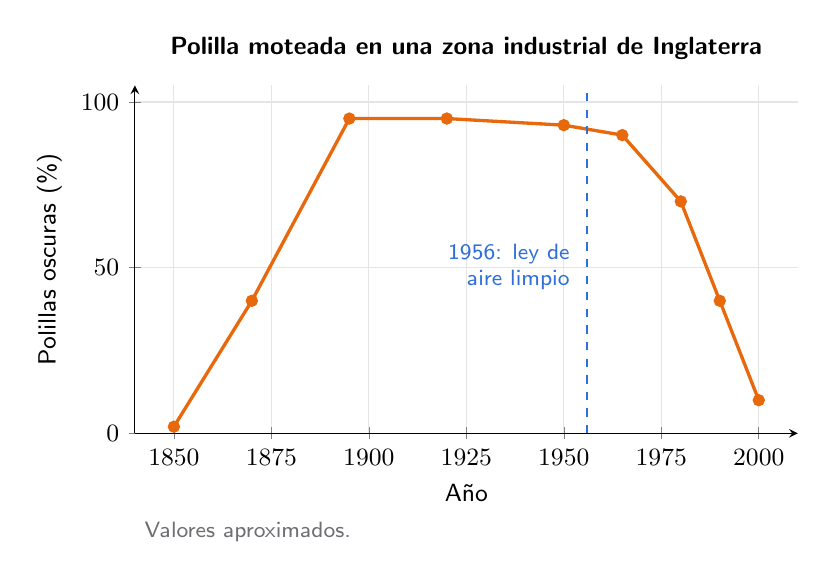
\begin{tikzpicture}[font=\small]
\begin{axis}[width=10cm,height=6cm,axis lines=left,grid=major,grid style={gray!20},
  xmin=1840,xmax=2010,ymin=0,ymax=105,xtick={1850,1875,1900,1925,1950,1975,2000},
  /pgf/number format/1000 sep={},
  xlabel={Año},ylabel={Polillas oscuras (\%)},title={Polilla moteada en una zona industrial de Inglaterra},
  title style={font=\small\bfseries}]
\addplot[nar,very thick,mark=*,mark options={scale=0.8,fill=nar}] coordinates {(1850,2)(1870,40)(1895,95)(1920,95)(1950,93)(1965,90)(1980,70)(1990,40)(2000,10)};
\draw[azul,dashed,thick] (axis cs:1956,0) -- (axis cs:1956,104);
\node[anchor=north east,align=right,font=\footnotesize,text=azul] at (axis cs:1954,60) {1956: ley de\\aire limpio};
\end{axis}
\node[anchor=north west,font=\footnotesize,text=gris] at (0,-1.0) {Valores aproximados.};
\end{tikzpicture}
\end{document}
